% AMO operators pseudocode for papers
% Compile with: pdflatex or xelatex (requires algorithm2e package)
\documentclass[a4paper]{article}
\usepackage[utf8]{inputenc}
\usepackage{amsmath,amssymb}
\usepackage[ruled,vlined,linesnumbered]{algorithm2e}
\usepackage{tikz}
\usetikzlibrary{arrows.meta,positioning,shapes.multipart,fit}
\DontPrintSemicolon
\SetKwInput{KwData}{Input}
\SetKwInput{KwResult}{Output}
\SetKwProg{Proc}{Procedure}{}{}
\SetKwFunction{FRepair}{RepairPipeline}
\SetKwFunction{FEval}{Evaluate}

\newcommand{\zeros}{\text{zeros}}
\newcommand{\varDim}{\text{varDim}}

\begin{document}

\title{Pseudocode: AMO Structure-Preserving Operators}
\author{(Extracted from PlatEMO A-amos implementation)}
\date{}
\maketitle

\noindent\textit{Notation: chromosome length $\varDim = 2n + m - 1$; genes $1..n$ merchants, $n{+}1..2n$ customers; $m{-}1$ delimiters ``0''; each merchant $s$ must appear before customer $s{+}n$.}

\noindent\textbf{Population initialization} is \emph{outside} \texttt{OperatorAMO}. In PlatEMO, \texttt{Problem.Initialization()} builds the first generation (see \texttt{A\_amos.m}). This PDF focuses on the operator module.

\begin{figure}[htbp]
\centering
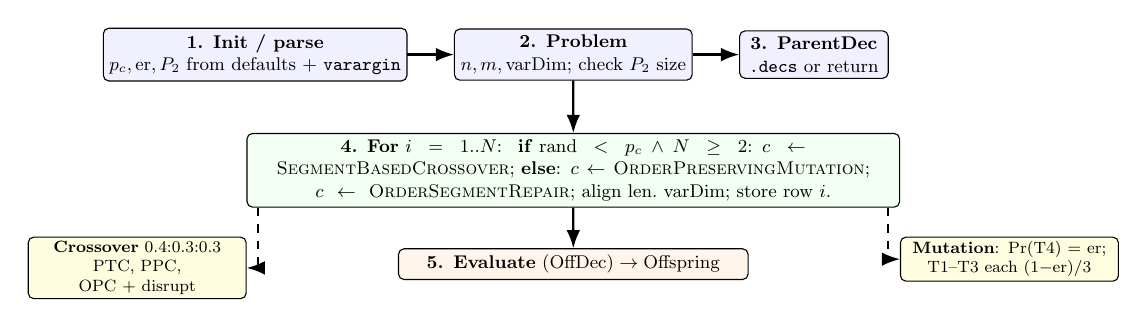
\begin{tikzpicture}[
  scale=0.74, transform shape,
  node distance=4mm and 6mm,
  box/.style={rectangle, draw, rounded corners=2pt, align=center, inner sep=3pt, minimum width=2.55cm, font=\small},
  small/.style={rectangle, draw, rounded corners=2pt, align=center, inner sep=2pt, font=\footnotesize},
  arr/.style={-Latex, thick}
]
% --- OperatorAMO top-level (compact horizontal) ---
\node[box, fill=blue!6] (parse) {\textbf{1. Init / parse}\\$p_c,\mathrm{er},P_2$ from defaults + \texttt{varargin}};
\node[box, right=8mm of parse, fill=blue!6] (prob) {\textbf{2. Problem}\\$n,m,\varDim$; check $P_2$ size};
\node[box, right=8mm of prob, fill=blue!6] (dec) {\textbf{3. ParentDec}\\\texttt{.decs} or return};
\node[below=9mm of prob, box, minimum width=11.2cm, fill=green!5, text width=10.8cm] (loop)
  {\textbf{4. For} $i=1..N$: \ 
  \textbf{if} $\mathrm{rand}<p_c \land N\geq 2$: $c\leftarrow\textsc{SegmentBasedCrossover}$;\ 
  \textbf{else}: $c\leftarrow\textsc{OrderPreservingMutation}$;\ 
  $c\leftarrow\textsc{OrderSegmentRepair}$; align len.\ $\varDim$; store row $i$.};
\node[box, below=7mm of loop, fill=orange!8, minimum width=6cm] (eval) {\textbf{5. Evaluate} $\FEval(\text{OffDec})\rightarrow\text{Offspring}$};
\draw[arr] (parse) -- (prob);
\draw[arr] (prob) -- (dec);
\draw[arr] (prob) -- (loop);
\draw[arr] (loop) -- (eval);
% --- fan-out ---
\node[small, below left=5mm and 0mm of loop.south west, fill=yellow!12, text width=3.6cm] (cx)
  {\textbf{Crossover} $0.4{:}0.3{:}0.3$\\PTC, PPC, OPC + disrupt};
\node[small, below right=5mm and 0mm of loop.south east, fill=yellow!12, text width=3.6cm] (mut)
  {\textbf{Mutation}: $\Pr(\mathrm{T4})=\mathrm{er}$;\\T1--T3 each $(1{-}\mathrm{er})/3$};
\draw[dashed, arr] (loop.south west) ++(0.2,0) |- (cx);
\draw[dashed, arr] (loop.south east) ++(-0.2,0) |- (mut);
\end{tikzpicture}
\caption{Overall framework of \texttt{OperatorAMO} (as implemented in \texttt{OperatorAMO.m}): parameter initialization, Problem fields, per-offspring genetic operator, unified segment repair, and batch evaluation. Side boxes summarize the three crossover modes and four mutation modes.}
\label{fig:operator-amo-framework}
\end{figure}

\begin{algorithm}[htbp]
\caption{OperatorAMO (complete procedure, matches \texttt{OperatorAMO.m})}
\KwData{Problem, \texttt{Parents} (with field \texttt{decs}), optional key-value list \texttt{varargin}}
\KwResult{\texttt{Offspring} = evaluated individuals}
$p_c \gets 0.5$; $\mathrm{er} \gets 0.25$; $P_2 \gets \emptyset$\;
\For{$\ell = 1$ \KwTo $\lfloor \mathrm{length}(\texttt{varargin})/2 \rfloor$}{
  $j \gets 2\ell-1$; $\text{key} \gets \mathrm{lower}(\texttt{varargin}(j))$; $\text{val} \gets \texttt{varargin}(j{+}1)$\;
  \uIf{\text{key} is \texttt{pc}}{$p_c \gets \text{val}$}
  \uElseIf{\text{key} is \texttt{er} \textbf{or} \texttt{explorationrate}}{$\mathrm{er} \gets \text{val}$}
  \uElseIf{\text{key} is \texttt{p2} / \texttt{extraparents} / \ldots}{$P_2 \gets \text{val}$}
}
$n \gets \texttt{Problem.n}$; $m \gets \texttt{Problem.m}$; $\varDim \gets \texttt{Problem.D}$\;
$\textit{ParentDec} \gets \texttt{Parents.decs}$\;
\If{$\textit{ParentDec}$ is empty}{\Return $\FEval(\textit{ParentDec})$ \tcp*{PlatEMO convention}}
\If{$P_2 \neq \emptyset$}{
  extract matrix $P_2^{dec}$ from $P_2$\;
  \If{sizes of $P_2^{dec}$ and $\textit{ParentDec}$ disagree}{\textbf{throw} size error\;}
}
\Else{$P_2^{dec} \gets []$\;}
$N \gets \mathrm{nrows}(\textit{ParentDec})$; allocate $\textit{OffDec} \in \mathbb{R}^{N \times \varDim}$\;
\For{$i = 1$ \KwTo $N$}{
  $p_1 \gets \textit{ParentDec}(i,:)$\;
  \eIf{$\mathrm{rand}() < p_c$ \textbf{and} $N \geq 2$}{
    \eIf{$P_2^{dec} \neq []$}{$p_2 \gets P_2^{dec}(i,:)$}{
      draw $p_2$ uniformly from $\textit{ParentDec}(\{1..N\}\setminus\{i\},:)$\;
    }
    $c \gets \textsc{SegmentBasedCrossover}(p_1,p_2,n,m,\varDim)$\;
  }{
    $c \gets \textsc{OrderPreservingMutation}(p_1,m,\varDim,n,\mathrm{er})$\;
  }
  $c \gets \textsc{OrderSegmentRepair}(c,n,m,\varDim)$\;
  enforce $\mathrm{length}(c)=\varDim$ (pad with zeros or truncate)\;
  $\textit{OffDec}(i,:) \gets c$\;
}
\Return $\FEval(\textit{OffDec})$\;
\end{algorithm}

\begin{algorithm}[htbp]
\caption{SegmentBasedCrossover}
\KwData{$p_1,p_2,n,m,\varDim$}
\KwResult{offspring $c$, strategy id $\in\{1,2,3\}$}
$r \gets \mathrm{rand}()$\;
\uIf{$r < 0.4$}{
  $c \gets \textsc{PositionTrackingCrossover}(p_1,p_2,n,m,\varDim)$ \tcp*{PTC}
}
\uElseIf{$r < 0.7$}{
  $c \gets \textsc{PairPriorityCrossover}(p_1,p_2,n,m,\varDim)$ \tcp*{PPC}
}
\Else{
  $c \gets \textsc{OrderPreservingCrossover}(p_1,p_2,n,m,\varDim)$ \tcp*{OPC}
}
trim / pad $c$ to $\varDim$; remove leading/trailing zeros\;
\If{$c = p_1$ \textbf{or} $c = p_2$}{
  $c \gets \textsc{ForceDisrupt}(c,n,m,\varDim)$ \tcp*{break clone}
}
\Return $c$\;
\end{algorithm}

\begin{algorithm}[htbp]
\caption{PositionTrackingCrossover (PTC)}
\KwData{valid parents $p_1,p_2$}
\KwResult{offspring $c$}
build position maps $\pi_1,\pi_2$ for genes $1..2n$\;
$\mathcal{K} \gets \{ k \in [1,\varDim{-}1] : k \text{ is safe for both } \pi_1,\pi_2\}$\;
\tcp{safe: no pair $(s,s{+}n)$ with $\pi(s)<k<\pi(s{+}n)$}
\If{$\mathcal{K} = \emptyset$}{\Return $p_1$\;}
sample $k \in \mathcal{K}$ uniformly\;
$c(1:k) \gets p_1(1:k)$; $U \gets$ multiset of genes in $c(1:k)$\;
$i \gets k{+}1$\;
\For{scan index $t$ from $1$ to $\varDim$}{
  $g \gets p_2(t)$\;
  \If{$g \notin U$}{
    \uIf{$g=0$}{append $g$; add to $U$\;}
    \uElseIf{$n < g \leq 2n$}{
      \If{merchant $(g{-}n) \in U$}{append $g$; add to $U$\;}
    }
    \Else{append $g$; add to $U$\;}
  }
  \If{filled up to $\varDim$}{\textbf{break}\;}
}
$c \gets \textsc{RepairSolution}(c,n,m,\varDim)$\;
\If{\textbf{not} \textsc{IsValid}$(c)$}{$c \gets \textsc{RepairOrder}(c,n)$\;}
$c \gets \textsc{RepairSegments}(c,n,m)$\;
\Return $c$\;
\end{algorithm}

\begin{algorithm}[htbp]
\caption{PairPriorityCrossover (PPC)}
\KwData{valid parents $p_1,p_2$}
\KwResult{offspring $c$}
\For{$s=1$ \KwTo $n$}{
  $\mathrm{pri}_1(s) \gets$ first index of $s$ in $p_1$\;
  $\mathrm{pri}_2(s) \gets$ first index of $s$ in $p_2$\;
  $\mathrm{merged}(s) \gets \min(\mathrm{pri}_1(s),\mathrm{pri}_2(s))$\;
}
sort merchants by increasing $\mathrm{merged}(s)$ $\rightarrow$ list $M$\;
initialize $c \gets \zeros(1,\varDim)$; write $M(1),M(2),\ldots$ into $c$ from the left\;
\ForEach{merchant $s$ in $M$}{
  find position $\ell$ of $s$ in $c$\;
  scan right from $\ell{+}1$: set first slot still $0$ to customer $s{+}n$\;
}
$c \gets \textsc{RepairSolution}(c,n,m,\varDim)$\;
\If{\textbf{not} \textsc{IsValid}$(c)$}{$c \gets \textsc{RepairOrder}(c,n)$\;}
$c \gets \textsc{RepairSegments}(c,n,m)$\;
\Return $c$\;
\end{algorithm}

\begin{algorithm}[htbp]
\caption{OrderPreservingCrossover (OPC)}
\KwData{valid parents $p_1,p_2$}
\KwResult{offspring $c$}
extract merchant visit orders $O_1,O_2$ (first occurrences, duplicates removed)\;
\If{$O_1$ or $O_2$ empty}{\Return $p_1$\;}
$f \gets \mathrm{randint}(1,|O_1|)$\;
$F \gets \mathrm{unique}([O_1(1:f),O_2(f{+}1:\text{end})],\text{stable})$\;
append missing merchants from $O_1 \cup O_2$ to $F$\;
\If{$F = O_1$ \textbf{and} $|F|\geq 2$}{swap two random positions in $F$\;}
build $c$ from $F$ exactly as in PPC (write merchants, then fill first zero after each)\;
$c \gets \textsc{RepairSolution}(c,n,m,\varDim)$\;
\If{\textbf{not} \textsc{IsValid}$(c)$}{$c \gets \textsc{RepairOrder}(c,n)$\;}
$c \gets \textsc{RepairSegments}(c,n,m)$\;
\Return $c$\;
\end{algorithm}

\begin{algorithm}[htbp]
\caption{OrderPreservingMutation}
\KwData{individual $x$, counts $m,n$, dimension $\varDim$, exploration rate $\rho$}
\KwResult{mutated $x'$}
split $x$ into segments $S_1..S_m$ by $m{-}1$ zeros\;
\uIf{$\mathrm{rand}() < \rho$}{
  $x' \gets \textsc{Type4\_SegSwap}(x,\{S_k\},m,n,\varDim)$ \tcp*{large step}
}
\Else{
  $t \gets \mathrm{randint}(1,3)$\;
  \uIf{$t=1$}{
    $x' \gets \textsc{Type1}(x)$ \tcp*{random merchant to segment head}
  }
  \uElseIf{$t=2$}{
    $x' \gets \textsc{Type2}(x)$ \tcp*{random customer to segment tail}
  }
  \Else{
    $x' \gets \textsc{Type3\_MoveDelimiter}(x)$ \tcp*{slide delimiter ``0''}
  }
}
fix length and zero count; \If{$x'=x$}{retry Type4 / intra-segment pair swap\;}
\Return $x'$\;
\end{algorithm}

\begin{algorithm}[htbp]
\caption{Mutation Type1: move random merchant to \emph{head} of its segment}
\KwData{individual $x$, segments $\{S_k\}$, delimiter index array $E$ (extended zero positions)}
\KwResult{$x'$}
$\mathcal{V} \gets \{ k : S_k \text{ contains some merchant in } \{1..n\}\}$\;
\If{$\mathcal{V}=\emptyset$}{\Return $x$\;}
sample $k \in \mathcal{V}$; let $\sigma \gets S_k$\;
pick random merchant gene $a$ from $\sigma$\;
remove $a$ from its position in $\sigma$; $\sigma' \gets [a,\sigma]$\;
$x' \gets x$; write $\sigma'$ back into positions $(E(k){+}1)..(E(k{+}1){-}1)$\;
\Return $x'$\;
\end{algorithm}

\begin{algorithm}[htbp]
\caption{Mutation Type2: move random customer to \emph{tail} of its segment}
\KwData{individual $x$, segments $\{S_k\}$, extended indices $E$}
\KwResult{$x'$}
$\mathcal{V} \gets \{ k : S_k \text{ contains some customer in } \{n{+}1..2n\}\}$\;
\If{$\mathcal{V}=\emptyset$}{\Return $x$\;}
sample $k \in \mathcal{V}$; $\sigma \gets S_k$\;
pick random customer $b$ from $\sigma$\;
remove $b$; $\sigma' \gets [\sigma, b]$\;
$x' \gets x$; write $\sigma'$ into segment $k$\;
\Return $x'$\;
\end{algorithm}

\begin{algorithm}[htbp]
\caption{Mutation Type3: slide one delimiter ``0'' (pair-safe boundaries)}
\KwData{$x$, segments $\{S_k\}$, $E$, counts $m,n,\varDim$}
\KwResult{$x'$}
\If{$m \leq 1$}{\Return $x$\;}
pick movable delimiter index $z \in \{1..m{-}1\}$ (adjacent segments nonempty)\;
$d \gets \mathrm{randint}(0,1)$ \tcp*{$0$: scan backward in left segment; $1$: forward in right}
\If{$d=0$}{
  $q \gets \textsc{TraverseForward}(x,E,z,S_z,n)$ \tcp*{first valid slot before a merchant}
}
\Else{
  $q \gets \textsc{TraverseBackward}(x,E,z,S_{z+1},n)$ \tcp*{first valid slot after a customer}
}
\If{$q<0$}{\Return $x$\;}
remove the old ``0'' at global index $E(z{+}1)$ from $x$; adjust $q$ if needed\;
insert ``0'' at global index $q$; pad/trim to $\varDim$\;
\Return $x'$\;
\end{algorithm}

\begin{algorithm}[htbp]
\caption{TraverseForward / TraverseBackward (Type3 helpers, sketch)}
\KwData{segment vector, delimiter context, $n$}
\KwResult{global index for new ``0'', or $-1$ if impossible}
\textsc{TraverseForward} scans the left segment from \emph{tail} to \emph{head}\;
\Indp
at each merchant $a$, let $C$ be customers in the already-scanned suffix\;
\lIf{$C$ is empty or $C \subseteq (\text{merchants scanned}\cup\{a\}){+}n$ \textbf{and} slot before $a$ is legal}{return that index}
\Indm
\textsc{TraverseBackward} scans the right segment from \emph{head} to \emph{tail}\;
\Indp
at each customer $c$, let $M$ be merchants in the already-scanned prefix\;
\lIf{$M$ is empty or $M \subseteq (\text{customers scanned}\cup\{c\}){-}n$ \textbf{and} slot after $c$ is legal}{return that index}
\Indm
\Return $-1$\;
\end{algorithm}

\begin{algorithm}[htbp]
\caption{Type4\_SegSwap (sketch)}
\KwData{segments $\{S_k\}$}
choose source $k_s$ with at least two merchant--customer pairs\;
pick random merchant $a$ in $S_{k_s}$ with both $a$ and $a{+}n$ present\;
remove $(a,a{+}n)$ from $S_{k_s}$ preserving order\;
choose target $k_t \neq k_s$; random insertion position in $S_{k_t}$\;
insert consecutive $(a,a{+}n)$\;
rebuild chromosome; \If{constraints violated}{\Return $x$ unchanged\;}
\Return rebuilt chromosome\;
\end{algorithm}

\begin{algorithm}[htbp]
\caption{Repair pipeline (abstract)}
\KwData{chromosome $c$}
$\textsc{EnsureNoZeroAtEnds}(c)$\;
$\textsc{RepairSegments}(c)$ \tcp*{move customers to merchant segments}
$\textsc{RepairSegmentSizes}(c,m)$ \tcp*{each segment has even length $\geq 2$}
pad/trim to $\varDim$\;
\Return $c$\;
\end{algorithm}

\end{document}
